%% 
%% Copyright 2007-2020 Elsevier Ltd
%% 
%% This file is part of the 'Elsarticle Bundle'.
%% ---------------------------------------------
%% 
%% It may be distributed under the conditions of the LaTeX Project Public
%% License, either version 1.2 of this license or (at your option) any
%% later version.  The latest version of this license is in
%%    http://www.latex-project.org/lppl.txt
%% and version 1.2 or later is part of all distributions of LaTeX
%% version 1999/12/01 or later.
%% 
%% The list of all files belonging to the 'Elsarticle Bundle' is
%% given in the file `manifest.txt'.
%% 
%% Template article for Elsevier's document class `elsarticle'
%% with harvard style bibliographic references
\documentclass[preprint,12pt,authoryear]{elsarticle}


%% Use the option review to obtain double line spacing
%% \documentclass[authoryear,preprint,review,12pt]{elsarticle}

%% Use the options 1p,twocolumn; 3p; 3p,twocolumn; 5p; or 5p,twocolumn
%% for a journal layout:
%% \documentclass[final,1p,times,authoryear]{elsarticle}
%% \documentclass[final,1p,times,twocolumn,authoryear]{elsarticle}
%% \documentclass[final,3p,times,authoryear]{elsarticle}
%% \documentclass[final,3p,times,twocolumn,authoryear]{elsarticle}
%% \documentclass[final,5p,times,authoryear]{elsarticle}
%% \documentclass[final,5p,times,twocolumn,authoryear]{elsarticle}

%% For including figures, graphicx.sty has been loaded in
%% elsarticle.cls. If you prefer to use the old commands
%% please give \usepackage{epsfig}
\graphicspath{{../plots/}}

%% The amssymb package provides various useful mathematical symbols
\usepackage{amssymb, amsmath}
\DeclareMathOperator*{\argmin}{arg\,min}
\DeclareMathOperator*{\argmax}{arg\,max}
\DeclareMathOperator*{\expd}{exp.}
%% The amsthm package provides extended theorem environments
\usepackage{amsthm}
\newtheorem{proposition}{Proposition}
\usepackage{hyperref}
\hyperbaseurl{}
\urlstyle{same}
\usepackage{caption}

%% The lineno packages adds line numbers. Start line numbering with
%% \begin{linenumbers}, end it with \end{linenumbers}. Or switch it on
%% for the whole article with \linenumbers.
%% \usepackage{lineno}

\journal{Operations Research Letters}

\begin{document}

\begin{frontmatter}

%% Title, authors and addresses

%% use the tnoteref command within \title for footnotes;
%% use the tnotetext command for theassociated footnote;
%% use the fnref command within \author or \affiliation for footnotes;
%% use the fntext command for theassociated footnote;
%% use the corref command within \author for corresponding author footnotes;
%% use the cortext command for theassociated footnote;
%% use the ead command for the email address,
%% and the form \ead[url] for the home page:
 \title{Dynamic parameter estimation in the nested multinomial logit choice model}
%% \tnotetext[label1]{}
 \author{Max Kapur\corref{cor1}}
 \ead{maxkapur@snu.ac.kr}
%% \ead[url]{home page}
\cortext[cor1]{This research is supported by a grant from Seoul Metro, which oversees the public transportation network in Seoul.}
% \affiliation{organization={Seoul National University}, city={Seoul}, country={South Korea}}
 \address{Seoul National University, Department of Industrial Engineering, 39-411, 1 Gwanak-ro, Gwanak-gu, Seoul 08826, Republic of Korea}
%% \fntext[label3]{}

\begin{abstract}
This paper considers dynamic parameter estimation in the nested multinomial logit choice model under a tight computational constraint. We propose an intuitive step rule that updates the parameters each time a new consumer choice is observed. Stochastic convergence is guaranteed under the Robbins--Monro condition, and numerical simulations demonstrate the technique's feasibility.
\end{abstract}

%%Graphical abstract
%\begin{graphicalabstract}
%%\includegraphics{grabs}
%\end{graphicalabstract}

%%Research highlights
%\begin{highlights}
%\item This paper presents a technique for estimating the parameters of the nested multinomial logit choice model in a dynamic computational setting with a tight data limit. 
%\item The technique is based on a legible step rule whose convergence is guaranteed by classical results in stochastic approximation.
%\item Numerical simulations demonstrate the technique's feasibility.
%\end{highlights}

\begin{keyword}
choice models \sep multinomial logit \sep dynamic parameter estimation
%% keywords here, in the form: keyword \sep keyword

%% PACS codes here, in the form: \PACS code \sep code

%% MSC codes here, in the form: \MSC code \sep code
%% or \MSC[2008] code \sep code (2000 is the default)

\end{keyword}

\end{frontmatter}

%% \linenumbers
%% main text


\section{Introduction}
In a recent paper, \cite{honguyen2021} articulate the need for \emph{dynamic} choice modeling that can incorporate new observations of consumer behavior without solving a full optimization problem over the perturbed dataset. That paper concerned nonparametric choice models, which are hard to estimate even in a static setting \cite[][]{rusmevichientong2006, farias2013}. On the other hand, while \emph{parametric} choice models cannot accommodate every distribution of consumer preference orders \cite[][]{keane1997}, they offer a substantial advantage in the computational tractability of both model fitting and assortment optimization tasks \cite[][]{bunch1987, davis2014}. To establish parity in the debate over the relative merits of parametric and nonparametric choice models, it is worth examining whether this tractability advantage is equally pronounced in the dynamic setting. 

The present paper answers in the affirmative by providing a dynamic estimation scheme for the multinomial logit choice model and its nested variant in a tightly constrained computational environment called the data stream. When a new observation of a consumer choice arrives, the technique proposed here updates the current parameter estimate according to an intuitive rule with a sequence of decreasing step sizes. We show that stochastic convergence is guaranteed under the Robbins--Monro condition. The convergence rate can be further improved by tuning step parameters and utilizing a rolling average. We also demonstrate the feasibility of the technique through numerical simulations.

This paper is structured as follows. Sections \ref{modeldescription} and \ref{staticestimation} establish the notation and preliminary results in choice modeling. Section \ref{dynamicestimation} describes the update step and shows that it is a Robbins--Monro algorithm. Finally, section \ref{computation} provides numerical results.

\section{The multinomial logit choice model and its nested variant} \label{modeldescription}
Consider a portfolio of \emph{products} $\mathcal{N} = \{1 \dots n\}$. A consumer is offered an \emph{assortment} $\mathcal{A} \subseteq \mathcal{N}$ of products to choose from. A \emph{choice model} defines the probability that the consumer will choose product $i$.

In the multinomial logit (MNL) choice model, each consumer $t$'s preference order over the products in $\mathcal{N}$ is determined by the sum of a systematic product preferability parameter $\delta_i$ and a noise term $\epsilon_{it}$. The noise terms have an iid extreme-value distribution, and the consumer chooses the product in $\mathcal{A}$ for which $\delta_i + \epsilon_{it}$ is greatest. It can be shown that the probability of a given consumer choosing product $i$ from the assortment $\mathcal{A}$ is
\begin{equation}\label{mnlchoiceprobability}
\operatorname{Pr}\left[\,\text{choose } i \;|\;\text{assortment }\mathcal{A}\,\right] =\frac{\exp \delta_i}{\sum_{j\in \mathcal{A}} \exp \delta_j}
\end{equation}
The value of this equation does not change when each $\delta_i$ is perturbed by the same constant; hence, we may impose the normalization rule $\sum_{i=1}^n \delta_i = 0$ without loss of generality. 

A known issue with the MNL choice model is the assumption that introducing a new item into the assortment does not affect the preferability of the other items in the assortment relative to one another. This assumption, known as the independence of irrelevant alternatives, is violated when some products are near substitutes. The \emph{nested} multinomial logit model (NMNL) addresses this issue by dividing the consumer’s decision into two stages. 

Under NMNL, the customer first chooses a \emph{nest} $k \in \{ 1 \dots m\}$, then chooses a product $i$ within the nest. Both choices are made using MNL. Each nest's preferability parameter is written $\sigma_k$, while the products within the nest have preferability parameters $\delta_{ki}$. For convenience, assume each nest contains $n$ products; hence the product portfolio is $\mathcal{N} = \{1\dots m\} \times \{1\dots n\}$. We can represent a given assortment $\mathcal{A}$ as a list of (nest, product) tuples $(k, i)$. The assortment may span the $m$ nests and $mn$ products in any way. Let $\mathcal{A}^{\text{nests}}$ denote the set of nests represented in the assortment $\mathcal{A}$, and let $\mathcal{A}_k^{\text{products}}$ denote the set of products that are in both nest $k$ and the assortment $\mathcal{A}$. Then the probability that a given customer chooses the product $(k, i)$ is
\begin{equation}\label{nmnlchoiceprobability}
\operatorname{Pr}\left[\,\text{choose } (k, i) \;|\;\text{assortment }\mathcal{A}\,\right] =\frac{\exp \sigma_k}{\sum_{l\in \mathcal{A}^{\text{nests}}} \exp \sigma_l} \cdot \frac{\exp \delta_i}{\sum_{j\in\mathcal{A}_{k}^{\text{products}}} \exp \delta_j}\end{equation}
where we assume without loss of generality that $\sum_{k=1}^m \sigma_k = 0$ and $\sum_{i=1}^n \delta_{ki} = 0, \forall k$. 





\section{Static parameter estimation for (N)MNL} \label{staticestimation}
Consider the static parameter estimation task for the MNL choice model. $T$ consumers, indexed by $t$, were shown assortments $\mathcal{A}_t \subseteq \mathcal{N}$ and asked to pick their favorite product $y_t$. For convenience, abbreviate the preferability parameter associated with consumer $t$'s choice from $\delta_{y_t}$ to $\delta_t$. Then the likelihood of the $m$ observations with respect to the parameters $\delta$ is
\begin{equation} \label{mnllikelihood}
L(\delta) = \prod_{t=1}^T \frac{\exp \delta_t}{\sum_{j\in \mathcal{A}_t} \exp \delta_j}
\end{equation}
and maximizing the concave function $\log L(\delta)$ yields a maximum likelihood estimate of the model parameters.

Now consider the NMNL choice model. Each consumer $t$ chooses a product from an assortment $\mathcal{A}_t$, and we may write the consumer's choice as $(x_t, y_t)$, where $y_t$ is the product chosen and $x_t$ is the nest to which $y_t$ belongs. Again, $\mathcal{A}_t$ may be written as a list of (nest, product) tuples $(k, i)$. Let $\mathcal{A}_t^{\text{nests}}$ denote the set of nests represented in the assortment $\mathcal{A}_t$, let $\mathcal{A}_{t}^{\text{products}}$ denote the set of products that are in both nest $x_t$ and the assortment $\mathcal{A}_t$, and abbreviate the parameters $\sigma_{x_t}$ and $\delta_{y_t}$ to $\sigma_t$ and $\delta_t$. Then the likelihood function is
\begin{equation}L(\sigma, \delta) = \prod_{t=1}^T \frac{\exp \sigma_t}{\sum_{l\in \mathcal{A}_t^{\text{nests}}} \exp \sigma_l} \cdot \frac{\exp \delta_t}{\sum_{k \in \mathcal{A}_{t}^{\text{products}}} \exp \delta_k}\end{equation}
which is concave in the logarithm.

Computational tools for static estimation of variants of the MNL choice model are widely available \cite[e.g.][]{croissantnd}.







\section{Parameter estimation in the data stream framework} \label{dynamicestimation}
The dynamic scheme considered in this paper estimates NMNL parameters in online setting called the data stream. In the data stream, we are allowed to store only our \emph{current} parameter estimate and a state variable $t$ representing the number of observations used to construct the current estimate. When a new observation arrives, we can update the stored variables, but we cannot store the observation itself. %A simple example of a parameter estimation scheme in the data stream framework is the updating sample mean $\bar x^{(t+1)} = \frac{1}{t+1} \left( x_{t+1} + t \bar x^{(t)}\right)$. This calculation eliminates the need to store past observations of the random variable $X$, and each update is $\mathcal{O}(1)$ instead of the $\mathcal{O}(t)$ operations required to recalculate the mean over the full dataset. The MNL parameter update described below offers an analogous computational advantage.

\subsection{The MNL parameter update}
First, consider MNL without nests. Suppose that customers arrive in the order $\{1 \dots T\}$, and let $\delta^{(t)}$ denote the parameter estimate when customer $t$ arrives. The new observation indicates that customer $t$ chose product $y_t$ from consideration set $\mathcal{A}_t$. Let $Z^{(t)}$ denote the $n$-vector with
\begin{equation}Z^{(t)}_i =
\begin{cases}
 - \frac{\exp \delta^{(t)}_i}{\sum_{j\in \mathcal{A}_t} \exp \delta^{(t)}_j}, \quad& i \in \mathcal{A}_t, i\neq y_t \\
1 - \frac{\exp \delta^{(t)}_i}{\sum_{j\in \mathcal{A}_t} \exp \delta^{(t)}_j} , \quad& i \in \mathcal{A}_t, i =  y_t \\
0, \quad & i \notin \mathcal{A}_t
\end{cases}
\end{equation}

We propose the following \emph{MNL parameter update.}
\begin{align} \label{mnlparameterupdate}
\delta^{(t+1)} = \delta^{(t)} + \frac{\alpha}{t^r} Z^{(t)}
\end{align}
$\alpha >0$ and $r \in (0, 1]$ are step parameters. The intuition behind this parameter update is as follows. Seeing that $y_t$ was chosen from $\mathcal{A}_t$, we 
\begin{itemize}
\item Increase the estimated preferability of the item that was picked,
\item Decrease the estimated preferability of items that were rejected, and
\item Leave unchanged the preferability of items not in the presented assortment.
\end{itemize}
Notice that $\sum_{i=1}^n \delta_i$ remains constant under the parameter update, because $\sum_i Z_i = 0$. The starting point $\delta^{(1)}$ may be chosen arbitrarily. 

\begin{proposition}\label{mnlupdateconverges} If the observations are drawn from an MNL choice model and each consideration set appears with nonzero probability, then the MNL parameter update \eqref{mnlparameterupdate} converges in expectation to the true parameters $\delta$. 
\end{proposition}

%\subsection{A brief example}
%Suppose the parameter estimate is $\delta^{(1)} = (-2, 1, 3, -2)$ when we observe a consumer choose item $y_1 = 4$ from the consideration set  $\mathcal{A}_1 = \{2, 4\}$. Then when $\alpha = 1$, 
%\begin{align}
%\delta_{\mathcal{A}_1}^{(1)} =  \begin{bmatrix}1\\ -2\end{bmatrix}, \qquad e_{y_1} = \begin{bmatrix}0\\1\end{bmatrix} 
%\end{align}
%and
%\begin{align}
%\delta_{\mathcal{A}_2}^{(2)} &= \begin{bmatrix}1\\ -2\end{bmatrix} +
%\frac{1}{1}\left(\begin{bmatrix}0\\ 1\end{bmatrix} - \frac{1}{e^1 + e^{-2}}\begin{bmatrix}e^1\\ e^{-2}\end{bmatrix}\right) =
%\begin{bmatrix}0.05 \\ -1.05 \end{bmatrix} \\
%\implies \quad \delta^{(2)} &= (-2, 0.05, 3, -1.05)
%\end{align}
%is the updated parameter estimate.

To prove Proposition \ref{mnlupdateconverges}, we must invoke a few canonical results.

\subsection{Convergence of gradient processes using decreasing step sizes}
Consider the multivariate root-finding problem 
\begin{equation}\text{find } \theta^*: F(\theta^*) = 0\end{equation}
and the iterative scheme 
\begin{equation} \label{decreasingsteps}
\theta^{(t+1)} = \theta^{(t)} + \frac{\alpha}{t^r} F\left(\theta^{(t)} \right)
\end{equation}
where $\alpha >0$ and $r \in (0, 1]$ are step parameters. When $F: \mathbb{R}^n \mapsto \mathbb{R}^n$ is Lipschitz continuous and its Jacobian is negative definite, such an iterative scheme converges to the root, if it exists. A familiar example occurs when using gradient ascent to maximize a strictly concave function whose gradient is $F$ \cite[e.g.][prop. 1.2.4]{bertsekas1999}. For the extension to root finding, we refer to equations 11.36--41 of \cite{nocedal2006}, which imply that $F$ is a descent direction for the sum of squares $f(\theta) = \sum_{i=1}^n F_i(\theta)^2$, where the minimum of $f$ coincides with the root of $F$.

\subsection{Stochastic convergence and Robbins--Monro algorithms}
Suppose that in the update step \eqref{decreasingsteps},  $F(\theta)$ is replaced by an \emph{experiment} $\hat F(\theta)$ satisfying $\mathbb{E}\left[\hat F(\theta)\right] = F(\theta)$. Then the same iterative scheme is called a \emph{Robbins--Monro algorithm}, and exhibits \emph{stochastic convergence}; that is, with probability one,
\begin{equation}\lim_{t\to \infty} \mathbb{E}\left[F\bigl(\theta^{(t)}\bigr)\right] = \theta^*\end{equation}
\cite{robbinsmonro1951} presented this result for univariate $F$; a more general result appears in \cite{tsitsiklis1994}. Many convergence rate results from the deterministic case also generalize to stochastic interpretations \cite[][\S10.4]{kushner1997}.

%A classic example of a Robbins--Monro algorithm is stochastic gradient descent, which replaces the sum of error terms in a loss function with the errors of a randomly chosen subset of samples. In fact, the MNL parameter update can be regarded as a form of stochastic gradient descent for the log likelihood function, because when the single observation $(\mathcal{A}_t, y_t)$ constitutes the full dataset, a maximum likelihood estimator for the preferability of the products in $\mathcal{A}_t$ is the vector $e_{y_t}$ with a one at $y_t$ and zeros elsewhere. We offer a somewhat more targeted argument, however, in the following subsection.

\subsection{Proof of Proposition \ref{mnlupdateconverges}}
To prove that the MNL parameter update is a Robbins--Monro algorithm, it suffices to show that the optimal parameters are the zero of some function $F$ whose Jacobian is negative definite, and that the parameter update accords with an experiment $\hat F$ which is alike in expectation.  

Let $\delta$ denote the current parameter estimate and let $\delta^*$ denote the true, unknown parameters of the underlying MNL choice model. When the probability of offering each consideration set $\mathcal{A}$ is $\operatorname{Pr[\mathcal{A}]} > 0$, then the expected value of $Z$ has, at each index,
\begin{align}
\mathbb{E}\left[Z(\delta)_i \right] &= \sum_{\substack{\mathcal{A} \in 2^{\mathcal{N}}: \\ i \in \mathcal{A}}}\operatorname{Pr}\left[\mathcal{A}\right] \cdot \mathbb{E}\left[Z(\delta)_i\;|\;\mathcal{A}\right] \\
&=   \sum_{\substack{\mathcal{A} \in 2^{\mathcal{N}}: \\ i \in \mathcal{A}}}\operatorname{Pr}\left[\mathcal{A}\right] \cdot \left(\operatorname{Pr}\left[\,\text{choose } i\;|\;\mathcal{A}\,\right] - \frac{\exp \delta_i}{\sum_{j\in \mathcal{A}} \exp \delta_j} \right) \\
&= \sum_{\substack{\mathcal{A} \in 2^{\mathcal{N}}: \\ i \in \mathcal{A}}}\operatorname{Pr}\left[\mathcal{A}\right] \cdot \left(\frac{\exp  \delta_i^*}{\sum_{j\in \mathcal{A}} \exp \delta_j^*} - \frac{\exp \delta_i}{\sum_{j\in \mathcal{A}} \exp \delta_j} \right) \\
&= 0
\end{align}
if and only if $\delta^* = \delta$. Hence, the counterpart to $F(\theta)$ is the expected value of the random function $Z(\delta)$, while the counterpart to the experiment $\hat F(\theta)$ is the realization $Z^{(t)}(\delta)$. Next, observe that the Jacobian of $\mathbb{E}\left[Z(\delta) \right]$ is negative definite: The first term of the summand is constant, and the second is identical in form to the gradient of the logarithm of the likelihood function given in Equation \eqref{mnllikelihood}, which is strictly concave. Thus, we conclude that the iterative procedure is a Robbins--Monro algorithm and converges in expectation to $\delta^*$. 

\subsection{The NMNL parameter update}
The NMNL parameter update is analogous to the MNL parameter update. Each new observation consists of a consideration set $\mathcal{A}_t$, a nest choice $x_t$, and a product choice $y_t$. Define $\mathcal{A}_t^{\text{nests}}$ and $\mathcal{A}_{t}^{\text{products}}$ as above, and let
\begin{align}
W^{(t)}_k &= \begin{cases}
 -  \frac{\exp \sigma^{(t)}_k}{\sum_{l\in \mathcal{A}_{t}^{\text{nests}}} \exp \sigma_l}, \quad & k \in \mathcal{A}_{t}^{\text{nests}}, k \neq x_t\\
1 -  \frac{\exp \sigma^{(t)}_k}{\sum_{l\in \mathcal{A}_{t}^{\text{nests}}} \exp \sigma_l}, \quad & k \in \mathcal{A}_{t}^{\text{nests}}, k = x_t\\
0, \quad & k \notin \mathcal{A}_{t}^{\text{nests}}
\end{cases} \\
Z^{(t)}_{ki} &= 
\begin{cases}
 - \frac{\exp \delta^{(t)}_i}{\sum_{j\in \mathcal{A}_t^{\text{products}}} \exp \delta^{(t)}_j}, \quad&k = x_t, i \in \mathcal{A}_t^{\text{products}}, i\neq y_t \\
1 - \frac{\exp \delta^{(t)}_i}{\sum_{j\in \mathcal{A}_t^{\text{products}}} \exp \delta^{(t)}_j} , \quad&k = x_t, i \in \mathcal{A}_t^{\text{products}}, i =  y_t \\
0, \quad & \text{otherwise}
\end{cases}
\end{align}
The parameters are updated as follows.
\begin{align}\label{nmnlparameterupdate}
\sigma^{(t+1)} &= \sigma^{(t)} + \frac{\beta}{t^r} W^{(t)} \\
\delta^{(t+1)} &= \delta^{(t)} +  \frac{\alpha}{t^r} Z^{(t)} 
\end{align}
$\beta, \alpha >0$ and $r \in (0, 1]$ are step parameters.

\begin{proposition} \label{nmnlupdateconverges}
If the observations are drawn from an NMNL choice model and each consideration set appears with nonzero probability, then the NMNL parameter update converges to the true parameters $\sigma$ and $\delta$.\end{proposition}

Propositions \ref{mnlupdateconverges} and \ref{nmnlupdateconverges} require that each consideration set appear with nonzero probability in order to ensure that the input data contains information about the relative preferability of all possible pairs of products. The full-support assumption may be relaxed to the requirement that the graph $\mathcal{G}$ is connected, where the nodes of $\mathcal{G}$ are the products $\mathcal{N}$, and $\mathcal{G}$ has an arc between $i$ and $j$ if and only if both products belong to a consideration set that appears with nonzero probability. Indeed, the numerical experiments below employ this weaker assumption.


\section{Computational examples} \label{computation}
We demonstrate the tractability of the dynamic parameter update through three simulations. The first simulation concerns the MNL case and is summarized in Figure \ref{param-est-dynamic-nonnested}, while the second concerns the NMNL case and is summarized in Figure \ref{param-est-dynamic-nested}. In both simulations, a small number of products was chosen to yield a legible graph; the parameter update formula is computationally tractable for much higher values of $n$ and $m$. The third simulation considers a larger product portfolio with NMNL choice, and it compares the accuracy of maximum likelihood estimation over a large dataset with the final estimate that results from treating the same observations as a data stream and applying the dynamic update. While the accuracy is necessarily lower in the latter case, it may be acceptable given the savings in computation time. In all cases, it is possible to obtain smoother convergence by taking a rolling average or tuning the step parameters $\alpha$, $\beta$, and $r$.

The Julia code for these simulations is available on Github at \url{https://github.com/maxkapur/MultinomialLogit}. 





\begin{figure}
\begin{center}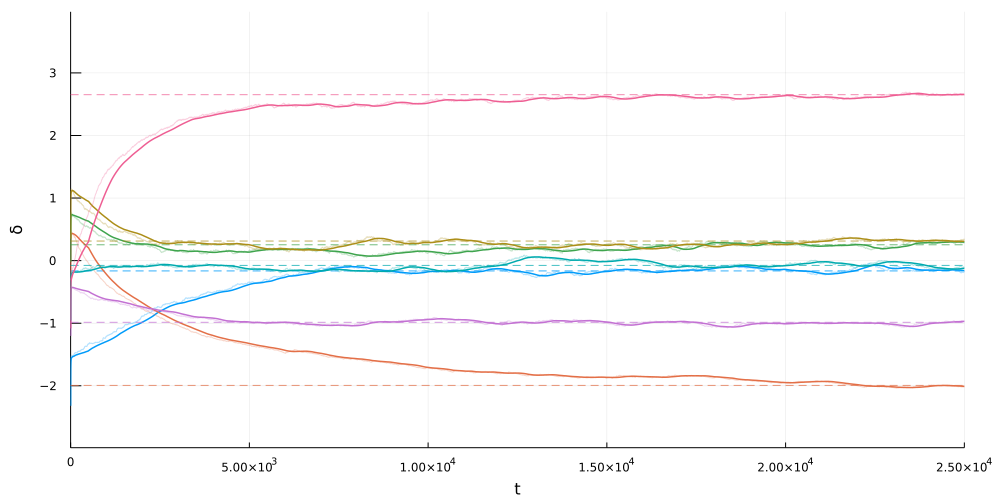
\includegraphics[width=\textwidth]{param-est-dynamic-nonnested.png}\end{center}
\captionsetup{singlelinecheck=off}
    \caption[.]{(Color.) Dynamic estimation of MNL choice parameters for a collection of $n = 7$ products. True preferability parameters $\delta$ and the initial estimate $\delta^{(1)}$ were drawn independently from a normal distribution and centered at zero. At $t = 1 \dots 25000$, a random assortment consisting of between two and five products was drawn, a consumer chose a product using the MNL choice model, and the parameter estimates were updated using Equation \ref{mnlparameterupdate}. The parameter estimate at each iteration is shown in a light stroke, while darker lines indicate a moving average over the previous 500 estimates. The step parameters are $\alpha = 0.01$ and $r = 0.05$.}
\label{param-est-dynamic-nonnested}
\end{figure}








\begin{figure}
\begin{center}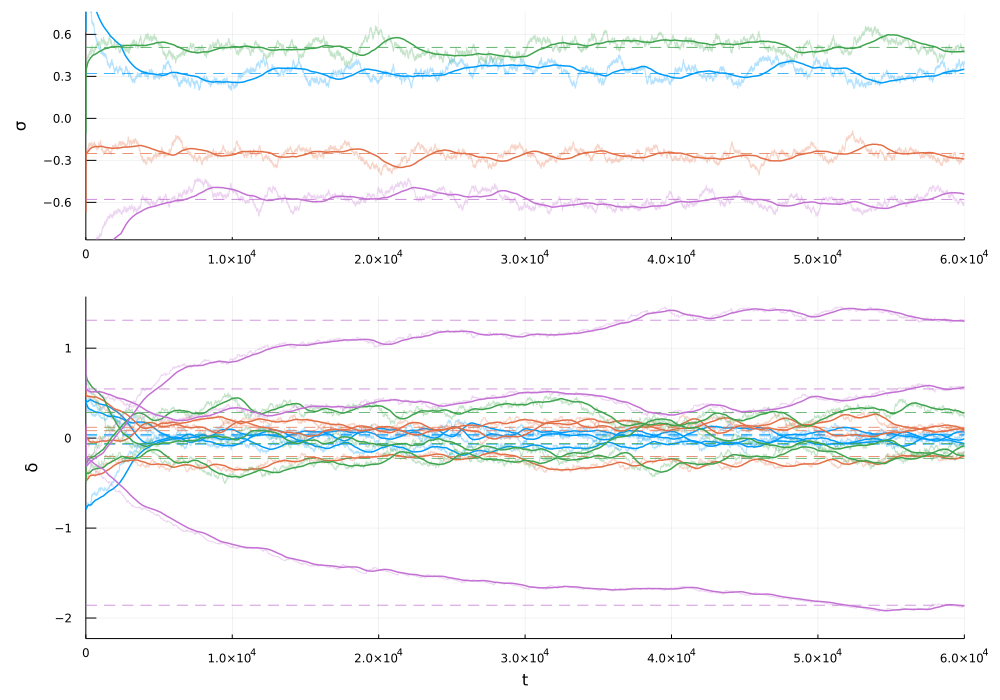
\includegraphics[width=\linewidth, ]{param-est-dynamic-nested.png}\end{center}
\captionsetup{singlelinecheck=off}
    \caption[.]{(Color.) Dynamic estimation of MNL choice parameters for a collection of $mn = 12$ products divided across $m=4$ nests. True preferability parameters $\sigma$ and $\delta$ as well as the initial parameter estimates were drawn independently from a normal distribution and centered at zero. At $t = 1 \dots 60000$, a random assortment consisting of between two and five products was drawn, a consumer chose a product using the NMNL choice model, and the parameter estimates were updated using Equation \ref{nmnlparameterupdate}. The parameter estimate at each iteration is shown in a light stroke, while darker lines indicate a moving average over the previous 1200 estimates. The step parameters are $\beta = 0.01$, $\alpha = 0.03$, and $r = 0.05$. The first pane shows the time series of $\sigma$ estimates, while the second shows the entries of $\delta$, color-coded by nest membership.}
\label{param-est-dynamic-nested}
\end{figure}





\begin{figure}
\begin{center}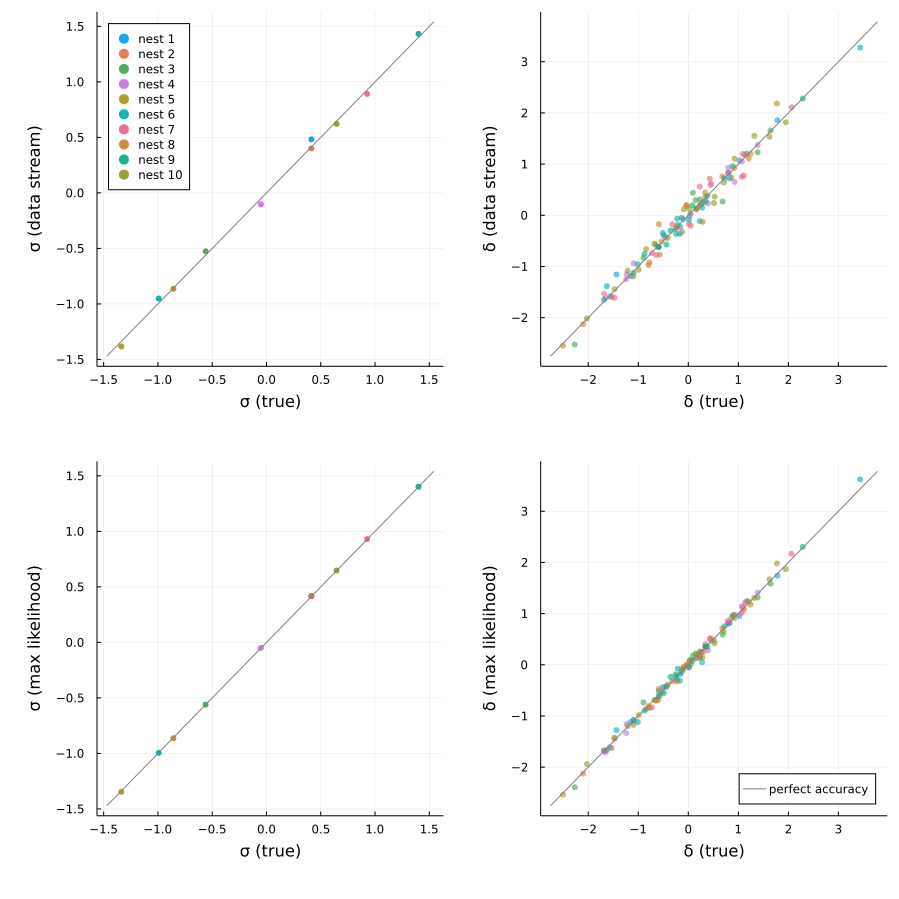
\includegraphics[width=\linewidth, ]{param-est-dynamic-nested-as-static.png}\end{center}
\captionsetup{singlelinecheck=off}
    \caption[.]{(Color.) Performance of the dynamic parameter estimate compared to maximum likelihood estimation. Preferability parameters for $mn = 120$ products divided into $m=10$ nests were drawn from the normal distribution and centered at zero. $T=500000$ assortments and consumer choices were generated according to the NMNL model. In the upper two panes, the observations were treated as a time series, and we report the estimate produced by the final iteration of the dynamic parameter update with step parameters $\beta = 0.01$, $\alpha = 0.03$, and $r = 0.05$. In the lower two panes, the parameters were estimated using maximum likelihood estimation. Dynamic parameter estimation offers acceptable accuracy at substantially lower computational cost.}
\label{param-est-dynamic-nested-as-static}
\end{figure}





\section{Conclusion}
Recent research in choice models has undergone two shifts in emphasis: one toward nonparametric choice models, and another toward the estimation thereof in a dynamic data setting. This paper has attempted to decouple these trends by considering the dynamic estimation of \emph{parametric} choice models in the MNL family.  Preliminary results suggest that the tractability advantage of parametric choice models is pronounced in the dynamic data setting. Whereas the dynamic algorithms suggested by \cite{honguyen2021} require solving a combinatorial subproblem at each iteration, the parameter update proposed here does not require any subiterative optimization, and each update's computational cost is proportional to the number of items in the assortment. Of course, all parametric choice models impose assumptions on the underlying distribution of consumer preference orders that may not be appropriate in all settings. Thus, the larger debate about the relative merits of parametric and nonparametric models is far from settled.

A natural extension of the ideas proposed here is the dynamic parameter estimation of other choice models within and beyond the MNL family.

%% The Appendices part is started with the command \appendix;
%% appendix sections are then done as normal sections
%% \appendix

%% \section{}
%% \label{}

%% If you have bibdatabase file and want bibtex to generate the
%% bibitems, please use
%%
%%  \bibliographystyle{elsarticle-harv} 
%%  \bibliography{<your bibdatabase>}

%% else use the following coding to input the bibitems directly in the
%% TeX file.qs

\begin{thebibliography}{00}

%% \bibitem[Author(year)]{label}
%% Text of bibliographic item
\bibitem[Bertsekas(1999)]{bertsekas1999}
Bertsekas, Dimitri P. 1999. \emph{Nonlinear Programming,} 2nd ed. Belmont, MA: Athena Scientific. 

\bibitem[Bunch(1987)]{bunch1987}
Bunch, David S. 1987. ``Maximum Likelihood Estimation of Probabilistic Choice Models.'' \emph{SIAM Journal on Scientific and Statistical Computing} 8(1): 56--70. {\url{https://doi.org/10.1137/0908006}}. 

\bibitem[Croissant(n.d.)]{croissantnd}
Croissant, Yves. ``Estimation of multinomial logit models in R: The \texttt{mlogit} Packages." {\url{https://www-eio.upc.es/teaching/madt/apunts/mlogit_teoria.pdf}}. 

\bibitem[Davis and Gallego and Topaloglu(2014)]{davis2014}
Davis, James M.,  Guillermo Gallego, and Huseyin Topaloglu. 2014. ``Assortment Optimization Under Variants of the Nested Logit Model.'' \emph{Operations Research} 62(2): 250--73. {\url{https://doi.org/10.1287/opre.2014.1256}}. 

\bibitem[Farias et al.(2013)]{farias2013}
Farias, Vivek F., Srikanth Jagabathula, and Devavrat Shah. 2013. “A Nonparametric Approach to Modeling Choice with Limited Data.” \emph{Management Science} 59(2): 305--22. {\url{https://doi.org/10.1287/mnsc.1120.1610}}. 

\bibitem[Ho-Nguyen and Kılınç-Karzan(2021)]{honguyen2021}
Ho-Nguyen, Nam and Fatma Kılınç-Karzan. 2021. ``Dynamic Data-Driven Estimation of Nonparametric Choice Models.'' \emph{Operations Research} 69(4): 1228--39. {\url{https://doi.org/10.1287/opre.2020.2077}}.

\bibitem[Keane(1997)]{keane1997}
Keane, Michael P. 1997. ``Current Issues in Discrete Choice Modeling." \emph{Marketing Letters} 8(3): 307--22. {\url{https://www.jstor.org/stable/40216456}}.

\bibitem[Kushner and Yin(1997)]{kushner1997}
Kushner, Harold J. and G. George Yin. 1997. \emph{Stochastic Approximation Algorithms and Applications.} New York: Springer. {\url{https://doi.org/10.1007/978-1-4899-2696-8}}.

\bibitem[Nocedal and Wright(2006)]{nocedal2006}
Nocedal, Jorge and Stephen J. Wright. 2006. \emph{Numerical Optimization,} 2nd ed. New York: Springer. {\url{https://doi.org/10.1007/b98874}}. 

\bibitem[Robbins and Monro(1951)]{robbinsmonro1951} 
Robbins, Herbert and Sutton Monro. 1951. ``A Stochastic Approximation Method." \emph{The Annals of Mathematical Statistics} 22(3): 400-407. {\url{https://doi.org/10.1214/aoms/1177729586}}. 

\bibitem[Rusmevichientong et al.(2006)]{rusmevichientong2006}
Rusmevichientong, Paat, Benjamin Van Roy and Peter W. Glynn. 2006. “A Nonparametric Approach to Multiproduct Pricing.” \emph{Operations Research} 54(1): 82--98. {\url{https://doi.org/10.1287/opre.1050.0252}}.

\bibitem[Tsitsiklis(1994)]{tsitsiklis1994}
Tsitsiklis, John. 1994. “Asynchronous Stochastic Approximation and Q-Learning.” \emph{Machine Learning} 16: 185--202.



\end{thebibliography}
\end{document}

\endinput
%%
%% End of file `elsarticle-template-harv.tex'.
